\section{Information Overload}

Information overload conveys the act of receiving \emph{too much information}. 
The problem is apparent in situations where decisional accuracy turns from improving with more information, to being hindered by too much irrelevant data \cite[p13]{Bjorkoy2010d}. 
Needness to say, this is a widespread phenomenon, with as many definitions as there are fields experiencing the problem. Examples include \emph{sensory overload}, \emph{cognitive overload} and \emph{information anxiety} \citep{Eppler2004}.

Two common tasks quickly become difficult in this situation:
Consuming content that is known by the user to be relevant can be drowned out by irrelevant noise.
Orthogonally, discovering new, interesting yet unknown content also becomes difficult because of the sheer amount of available content.
Finding contemporary examples is not difficult:

\begin{itemize*}
  \item Missing important news articles that get drowned out by irrelevant content.
  \item Forgetting to reply to an email as new messages keep arriving.
  \item Discovering sub-par movies because those most relevant are never discovered.
\end{itemize*}

The overload is often likened to a \emph{paradox of choice}, as there may be no problem acquiring the relevant information, but rather identifying this information once acquired. As put by \cite{Edmunds2000}: "The paradox --- a surfeit of information and a paucity of useful information."
While normal cases of such overload typically result in feelings of being overwhelmed and out of control, \cite{Bawden2008} points to studies linking extreme cases to various psychological conditions related to stressful situations, lost attention span, increased distractibility and general impatience.

\cite{Kirsh2000} argues that "the psychological effort of making hard decisions about \emph{pushed} information is the first cause of cognitive overload." 
According to \citeauthor{Kirsh2000}, there will never be a fully satisfiable solution to the problem of overabundant information, 
but that optimal environments can be designed to increase productivity and reduce the level of stress through careful consideration of the user's needs. 
In other words, to solve the problems of information overload and content discovery, applications must be able to individually adapt to each user. 

An insightful perspective on information overload comes from the study of attention economy. 
In this context human attention is seen a scarce commodity, offset by how much irrelevant noise is present at any given time. 
Attention can then be defined as "... focused mental engagement on a particular item of information. 
Items come into our awareness, we attend to a particular item, and then we decide whether to act" 
\citep{Davenport2001}. 
To evade information overload is then to maximize available attention, allowing more focus on the most important items of an interface.

\begin{wrapfigure}{rt}{0.4\textwidth}
  \vspace{-20pt}
  \begin{center}
    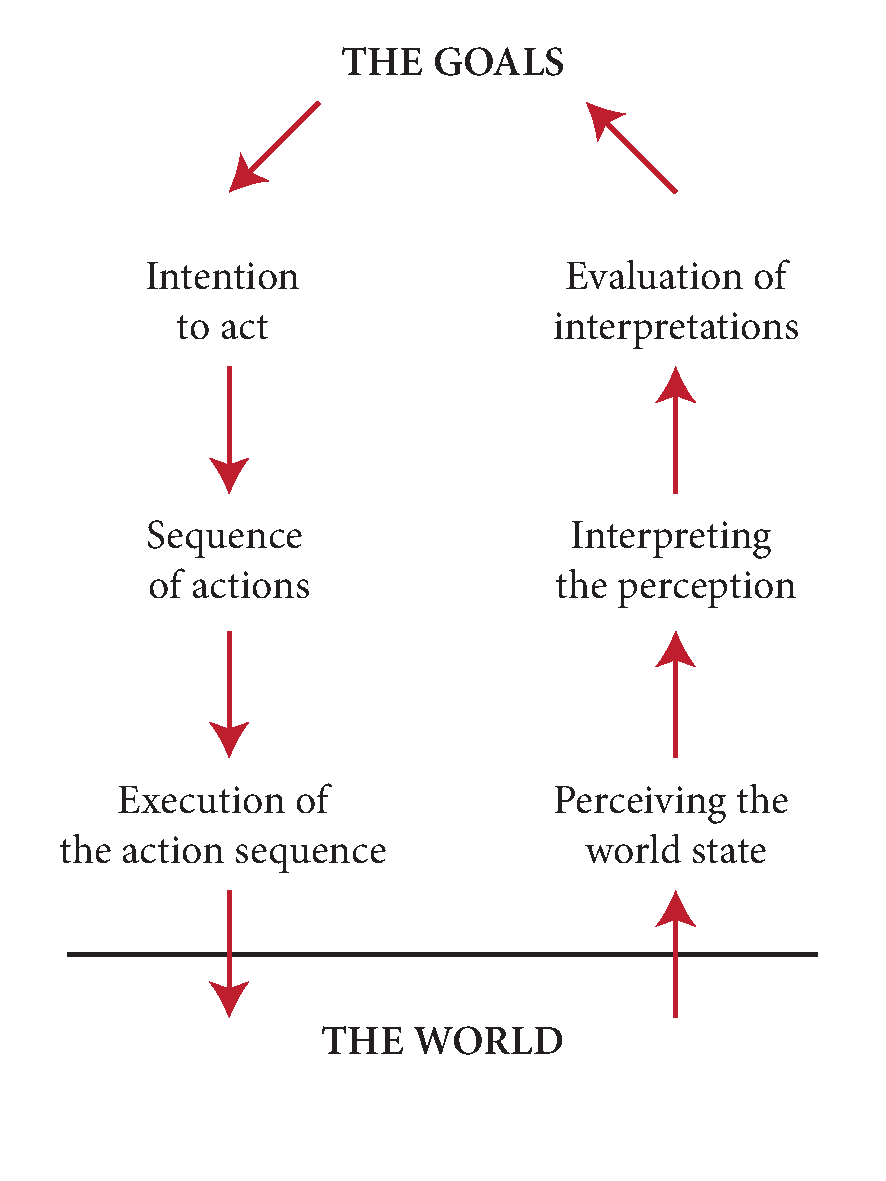
\includegraphics[width=0.4\textwidth]{../graphics/seven-stages.pdf}
    \vspace{-20pt}
    \caption[The Seven Stages of Action]{Stages of Action}
  \end{center}
  \label{fig:seven-stages}
  \vspace{-20pt}
\end{wrapfigure}

Conceptual models used in interaction design can help us see when and where information overload interferes with the user experience. 
\cite{Norman1988} advocates a model called the seven stages of action, describing how each user goes through several states while using a system
(see Figure \ref{fig:seven-stages}, adapted from \citeauthor{Norman1988}). 
First, the user forms a goal and an intention to act. The user then performs a sequence of actions on the world (the interface)
 meant to align the perceived world and the goals. After performing a set of actions, the new world state is evaluated and perceived. 
At last, the user evaluates the perception and interpretation of the world in accordance with the original goal.

As apparent from this model, information overload can interfere both before and after any action is taken. 
For example, if the application presents too much content, or presents content in a confusing manner, 
it can be difficult for the user to identify which actions that would help achieve the current goal. 
Likewise, after actions are taken, the new world state can suffer the same shortcomings of overwhelming scope or lack of presentations, 
leading to information overload. 
This precludes the user from properly evaluating the resulting application state. 

In short, an application interface can fail both before and after a user tries to interact with it.
Information overload happens throughout the interaction process, which is important to know when considering possible solutions.

\subsection{Online Overload}

The Web is a common source of information overload, 
and presents a good example of when and how the problem occurs.

Online information overload is especially pervasive when considering \emph{content aggregating websites}, 
i.e. sites that collate information from multiple other sites and sources. 
Online information retrieval (i.e. search engines), fall into this category, as does
online newspapers, feed readers and portal websites.
As mentioned, the wealth and scope of data are natural culprits of online overload, 
as well as the varying qualities of websites publishing the information. 

Graph theory presents applicable models of the Web that characterize how people navigate between websites, 
and show how content aggregators form important hubs in the network. 
These models also show a theoretical foundation for why information overload occurs.
In the Web graph, nodes correspond to websites and
directed edges between nodes are links from one page to another. The \emph{degree} of a node is defined as its number of edges.

The Internet has the properties of a \emph{small-world network} \citep{Newman2000}, 
a type of random graph, where most nodes are not neighbors, but most nodes are reachable through a small number of edges (See Figure \ref{fig:swn}). 
This is because of important random shortcuts differentiating the graph from a regular lattice. 
The graph is not  random, but neither is it completely regular.
As described by \citet[p37]{Barabasi2003}, the average number of outbound links from a webpage is around 7.
From the first page, we can reach 7 other pages. From the second, 49 documents can be reached. 
After 19 links have been traversed, about $10^{16}$ pages can be reached (which is more than the actual number of existing web pages, since loops will form in the graph).
%\footnote{The concept of small-world networks came from the observation that there is often a surprisingly short minimum distance between nodes in an average graph. This is called the small world phenomenon, and is often mentioned alongside the concept of "six degrees of separation", popularized in a play by John Guare. This concept states that no person is on average more than six social links removed from any other person on earth.}

\begin{figure}[t]
  \begin{framed}\centering
  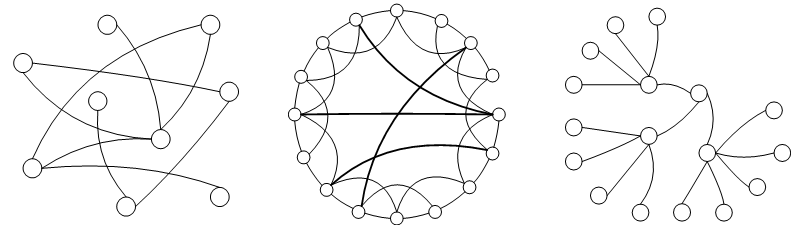
\includegraphics[width=\textwidth]{../graphics/graphs}
  \caption[Complex Networks]{
    Complex Networks,
    from the left: A \emph{random} network, a \emph{small-world} network and a \emph{scale-free} network 
    (which is a type of  small-world network). Figure adapted from \cite{Huang2005}.} 
  \label{fig:swn}
\end{framed}\end{figure}

The high degree of the Web graph would suggest that finding an optimal path to your desired page is quite difficult. 
Yet, while it is true that finding the \emph{optimal path} is hard, finding \emph{a good path} is not that big a challenge. 
When people browse the Web, links are not followed blindly --- we use numerous different heuristics to evaluate each link, often resulting in a quite good path to where we want to go. 
So why is the Web still quite challenging to navigate?

As discovered by \cite{Albert1999}, the Web also exhibits properties of a \emph{Scale-Free Network} (\smallcaps{SFN}). 
They found that in some natural observed networks, there exists a small number of nodes with an extremely high degree. 
This is also true on the Web --- some websites have a huge number of outbound links. 
For comparison, while a random network is similar to a national highway system, with a regular number of links between major cities, scale-free networks are more like an air traffic system, with central hubs connecting many less active airports \citep[p71]{Barabasi2003}.

These highly connected nodes, called \emph{hubs}, are not found in small-world networks or random graphs. As demonstrated by the presence of hubs, the degree distribution of a scale-free network follows a power law, 
$P(k) \sim k^{-\gamma}$, 
where $P(k)$ is the probability of a node having k connections and $\gamma$ is a constant dependent on the type of network, typically in the range $2 < \gamma < 3$. 
Since the Web has directed edges,
we have two power laws:
$P_{in}(k) \sim k^{-\gamma_{in}}$ and 
$P_{out}(k) \sim k^{-\gamma_{out}}$.

\cite{Albert1999} describes a number of studies placing the $\gamma$ values for the Web in the $[2,3]$ range, 
with $\gamma_{out}$ being slightly higher than $\gamma_{in}$. 
Both these probabilities exhibit power tails (or long tails). 
In other words, a few important nodes have a huge number of inbound and outbound links --- the hubs. 
\citet[p86]{Barabasi2003} proposed that hubs emerge in a scale-free networks because of two factors:
(1) Growth: Nodes are added to the network one by one, for example when new websites are added to the Internet.
(2) Preferential attachment: When new nodes are created, they connect to existing nodes. The probability that the new node will connect to an existing node is proportional to the number of links the existing node has. In other words, older, more established and central nodes are preferred neighbors.

This is called the Barab\'{a}si-Albert model \citep{Albert1999}, 
and the probability for a new node connecting to an existing node is given by $\prod k_i$ in Equation \ref{eq:albert:prob}, 
where $k_i$ is the number of links pointing to node $i$. 

\begin{equation}\label{eq:albert:prob}
  \prod_{i} k_i  = \frac{k_i}{\sum_{j}^N k_j}
\end{equation} 

Search engines, social link aggregators, news portals, et cetera are all hubs of the Internet, emerging from the preferential 
link attachment of newly created nodes. 
Factor in the existence of multiple sub-graphs, or continents, and we can intuitively see that navigating the Web is not as 
easy as it might appear from simple models.

What does seem clear is that these content aggregating hubs are prime candidates for overwhelming their users with information. 
The fundamental observed structure of the Web creates the need for information brokers that link the net together, 
and the need for techniques to display a lot of data --- adapted to each user and each item. 

So far we have established that information overload is a pervasive problem, especially on the web.
The question now becomes how to best solve this issue. 
This is where user modeling comes in.

